% The LIPIcs document class is used for many conferences in Computer Science.
% Refer to the templateLIPIcs folder for further information and examples.
\documentclass{lipics-v2021}

% Add your packages here.
\usepackage{amsthm}
\usepackage{hyperref}
\usepackage{booktabs}
\usepackage{caption}
\usepackage{subcaption}
\usepackage{tikz}
\usetikzlibrary{positioning,arrows.meta}

\newtheorem{question}{Question}

\newcommand{\todo}[1]{{\color{blue}TODO #1}}

\nolinenumbers

\title{Orientable Binary Tori with Single-Error Detection and a Self-Locating Jigsaw Puzzle}
\titlerunning{Orientable Binary Tori with Single-Error Detection}
\author{Tirthesh Jani}{Lakehead University, Canada}{tjani@lakeheadu.ca}{}{}
\authorrunning{T. Jani}
\Copyright{Tirthesh Jani}

\ccsdesc[500]{Mathematics of computing~Combinatorics}
\ccsdesc[300]{Mathematics of computing~Combinatorial algorithms}
\ccsdesc[300]{Computing methodologies~Computer vision}

\keywords{de Bruijn torus, orientable array, window distance, Hamming distance, position sensing, SAT solving, local search, jigsaw puzzle, robot vision}

\begin{document}

\maketitle

\begin{abstract}
A binary de Bruijn torus is an $R$-by-$C$ array of bits that wraps around in both directions and in which every binary $u$-by-$u$ array appears exactly once as a window.
A camera that reads one window can therefore determine its position on the torus.
This method fails when the camera is rotated by an unknown quarter turn, or when one cell is read incorrectly, because the rotated or altered window also appears at another position.

Burns and Mitchell (1993) defined 4-orientable arrays, in which all windows and all of their quarter turns are distinct.
Berkowitz and Kopparty (2016) studied arrays in which any two windows differ in at least $d$ cells.
We found no published binary torus that has both properties.

In this paper we study binary tori in which the $u$-by-$u$ windows and their quarter turns pairwise differ in at least two cells.
We call these \emph{strong-form} tori.
We prove an upper bound on their size that is half of the Burns--Mitchell bound when $u$ is odd.
We show by exhaustive computation that the largest strong-form torus for $3$-by-$3$ windows has $36$ cells, whereas 4-orientable tori with $85$ cells exist.
We construct a $256$-by-$256$ strong-form torus for $5$-by-$5$ windows by local search.
Finally, we use this torus in a two-sided jigsaw puzzle in which the back of each piece carries a $6$-by-$6$ patch of the torus, and we describe planned experiments in which a Reachy Mini robot reads a piece and reports its row, its column and its rotation.
\end{abstract}


\section{Introduction}
\label{sec:intro}

\subsection{De Bruijn Tori and Position Sensing}
\label{sec:intro_tori}

A binary de Bruijn torus is a two-dimensional generalization of a de Bruijn sequence.
It is an $R$-by-$C$ array of bits that is doubly periodic (i.e., it wraps around horizontally and vertically) and in which every binary $r$-by-$c$ array appears exactly once as a window.
Fan, Fan, Ma, and Siu constructed binary de Bruijn tori for every window size \cite{fan85debruijn}.
In this paper we consider square windows of size $u$-by-$u$.

De Bruijn tori are used for position sensing.
If the torus is printed on a surface, then a camera that reads a single window can look the window up in a table and obtain its position.
For example, the Dothraki tracking system prints a binary de Bruijn torus of size $8192$-by-$4096$ with $5$-by-$5$ windows, and a camera below each tracked object reads a small part of the pattern \cite{schusselbauer2021dothraki}.

\subsection{Unknown Orientation and Misread Cells}
\label{sec:intro_problems}

Position sensing with a de Bruijn torus assumes that the camera knows its orientation and that it reads every cell correctly.
A de Bruijn torus does not protect against a failure of either assumption.
The torus contains every binary $u$-by-$u$ array, so a window that has been rotated by a quarter turn is equal to the window at some other position, and so is a window in which one cell has been changed.
In both cases the table lookup succeeds and returns an incorrect position (see Example \ref{ex:debruijn}).

There are two ways to address this.
The first is to add checks to the decoder.
Dothraki reads a $6$-by-$6$ patch, tries all four orientations, and accepts a position only if the four overlapping $5$-by-$5$ windows of the patch are consistent \cite{schusselbauer2021dothraki}.
Schmid, Lippl, and Wimmer instead train a convolutional neural network to estimate the rotation of a camera image of such a torus before decoding, and the network determines the rotation only up to a quarter turn \cite{schmid2022determining}.
The second is to restrict the pattern.
Burns and Mitchell define an array to be \emph{4-orientable} if all of its windows and all of their quarter turns are distinct, so that a single window determines both position and orientation \cite{burns1993coding}.
Berkowitz and Kopparty study arrays in which any two windows differ in at least $d$ cells, so that up to $d-1$ incorrect cells can be detected \cite{berkowitz2016robust}.
The work on orientable arrays does not require a distance between windows, and the work on window distance assumes that the orientation is known.
We did not find a published periodic binary array in which all windows and their quarter turns are pairwise distinct and differ in at least two cells (see Section \ref{sec:background}).

\subsection{A Self-Locating Jigsaw Puzzle}
\label{sec:intro_jigsaw}

We also consider an application in which both problems occur.
Suppose that a jigsaw puzzle has a picture on the front and a binary pattern on the back.
If each piece carries a different part of a position-sensing pattern, then a camera can read the back of one piece and determine where the piece belongs.
A piece is held in front of the camera at an arbitrary rotation, and cells can be misread because of lighting, blur and perspective.
The reader therefore needs both the orientation and some protection against misread cells.

Existing computational approaches to jigsaw puzzles place a piece by comparing it with other pieces.
When the orientation of a piece is unknown, these approaches must also recover it.
\todo{Add citations for computational jigsaw solvers.}
In our puzzle each piece is located from its own pattern, without reference to any other piece.
We read the pieces with a Reachy Mini robot.\footnote{\url{https://github.com/pollen-robotics/reachy_mini}}

\subsection{Our Results}
\label{sec:intro_results}

We say that a binary torus is \emph{strong-form} for $u$-by-$u$ windows if any two of its windows, in any of their four orientations, differ in at least two cells (see Definition \ref{def:strong}).
A strong-form torus is 4-orientable, and a window with exactly one incorrect cell does not match any window in any orientation, so the error is detected.
In this paper we ask the following research questions.

\begin{question} \label{quest:size}
What is the maximum number of cells in a strong-form binary torus with $u$-by-$u$ windows?
\end{question}

\begin{question} \label{quest:cost}
How does this maximum compare with the maximum for 4-orientable binary tori, and is the difference explained by the counting bounds?
\end{question}

\begin{question} \label{quest:reader}
Does a strong-form pattern reduce the number of incorrect positions that a camera with unknown orientation reports, compared with a 4-orientable pattern of the same size?
\end{question}

We answer Question \ref{quest:size} exactly for $u=3$ and we give lower and upper bounds for $u=4$ and $u=5$.
The upper bound is the following theorem, which is proved in Section \ref{sec:bounds}.
For comparison, Burns and Mitchell prove that a 4-orientable binary torus has at most $(2^{u^2} - 2^{\lceil u^2/2 \rceil})/4$ cells \cite[Lemma~19]{burns1993coding}.

\begin{theorem} \label{thm:bound}
A strong-form binary torus with $u$-by-$u$ windows has at most $(2^{u^2-1} - 2^{(u^2-1)/2})/4$ cells if $u$ is odd, and at most $2^{u^2-2}$ cells if $u$ is even.
\end{theorem}

For odd $u$ the bound in Theorem \ref{thm:bound} is exactly half of the Burns--Mitchell bound.
For even $u$ the ratio of the two bounds is $2 - 2^{1-u^2/2}$, which is approximately $1.992$ for $u=4$.

\begin{theorem} \label{thm:exact3}
The maximum number of cells in a strong-form binary torus with $3$-by-$3$ windows is $36$.
A strong-form torus of size $R$-by-$C$ with $R \leq C$ exists if and only if $(R,C)$ is one of $(2,3)$, $(3,3)$, $(3,4)$, $(3,5)$, $(3,6)$, $(3,9)$, $(3,12)$ and $(6,6)$.
\end{theorem}

\begin{theorem} \label{thm:exist5}
There is a strong-form binary torus of size $256$-by-$256$ with $5$-by-$5$ windows.
\end{theorem}

Theorems \ref{thm:exact3} and \ref{thm:exist5} are computational results.
Theorem \ref{thm:exact3} was obtained with a SAT solver and confirmed by a separate exhaustive search (Section \ref{sec:exact}).
Theorem \ref{thm:exist5} was obtained by local search, and the resulting torus was checked directly (Section \ref{sec:constructions}).
Table \ref{tab:sizes} summarizes the bounds and the largest known tori.

\begin{table}[htbp]
\centering
\small
\begin{tabular}{@{}lrrrr@{}}
\toprule
 & \multicolumn{2}{c}{Upper bound (cells)} & \multicolumn{2}{c}{Largest known torus (cells)} \\
Window & 4-orientable & Strong-form & 4-orientable & Strong-form \\
\midrule
$3$-by-$3$ & $120$ & $60$ & $85$ ($5$-by-$17$) & $36$ (maximum) \\
$4$-by-$4$ & $16{,}320$ & $8{,}192$ & $4{,}096$ ($64$-by-$64$) & $441$ ($21$-by-$21$) \\
$5$-by-$5$ & $8{,}386{,}560$ & $4{,}193{,}280$ & $1{,}327{,}104$ ($1152$-by-$1152$) & $65{,}536$ ($256$-by-$256$) \\
\bottomrule
\end{tabular}
\caption{Upper bounds and largest known binary tori for each window size.
The 4-orientable upper bounds are from Burns and Mitchell \cite{burns1993coding} and the strong-form upper bounds are from Theorem \ref{thm:bound}.
The strong-form entry for $3$-by-$3$ windows is the exact maximum (Theorem \ref{thm:exact3}).
All other entries in the last two columns are lower bounds found by search.}
\label{tab:sizes}
\end{table}

We give a partial answer to Question \ref{quest:cost} for $u=3$.
The two upper bounds differ by a factor of $2$, but the maximum sizes differ by a factor between $85/36 \approx 2.36$ and $120/36 \approx 3.33$.
The cost of adding error detection is therefore larger than the counting bounds predict.
Exhaustive searches on arrays that do not wrap around suggest that the additional loss is caused by the requirement that the array is periodic (Section \ref{sec:exact}).
For $u=4$ and $u=5$ we only have search results, which are consistent with this conclusion but do not establish it.

Question \ref{quest:reader} is addressed by experiments.
We describe the jigsaw puzzle and its reading system in Section \ref{sec:jigsaw} and the experiments in Section \ref{sec:experiments}.
A preliminary computation shows that a decoder that checks four overlapping windows detects single misread cells even when the pattern is not strong-form.
For this reason the experiments vary the pattern and the decoder independently.
\todo{State the answer to Question \ref{quest:reader} when the experiments are complete.}

\subsection{Outline}
\label{sec:intro_outline}

Section \ref{sec:background} covers previous work and related work.
Section \ref{sec:preliminaries} gives definitions, examples and the limitations of the study.
Section \ref{sec:bounds} proves the upper bound in Theorem \ref{thm:bound}.
Section \ref{sec:exact} presents the exact results for $3$-by-$3$ windows.
Section \ref{sec:constructions} presents two algebraic constructions and the local search for larger windows.
Section \ref{sec:jigsaw} describes the self-locating jigsaw puzzle and the reading system.
Section \ref{sec:experiments} describes the experiments and their results.
Section \ref{sec:final} concludes with final remarks including open problems.


\section{Background}
\label{sec:background}

In this section we review the previous work on de Bruijn tori, orientable arrays and window distance.
Then we discuss related work on printed marker patterns, structured light and computational jigsaw puzzles.
Finally, we state the research problem.

\subsection{Previous Work}
\label{sec:background_previous}

\subparagraph*{De Bruijn tori.}
Fan, Fan, Ma, and Siu constructed binary de Bruijn tori for every window size \cite{fan85debruijn}.
Cock generalized the construction to larger alphabets \cite{cock1988toroidal}.
Etzion constructed perfect maps from perfect factors \cite{etzion1988constructions}, and Paterson proved that the necessary conditions on the parameters of a binary perfect map are also sufficient \cite{paterson1994perfect}.
Hurlbert and Isaak resolved most cases with square windows over larger alphabets \cite{hurlbert1993bruijn,hurlbert1995new}.
More recent constructions include tori built from alternating de Bruijn sequences \cite{kreitzer2024alternating} and nested perfect arrays \cite{becher2024nested}.
Decoding algorithms, which compute the position of a given window, were given by Mitchell and Paterson \cite{mitchell1994decoding}, by Shiu for the arrays of Fan et al.\ \cite{shiu1997decoding}, and by Horan and Stevens \cite{horan2016locating}.
Each of these arrays contains every window of its size.
Consequently, it contains every quarter turn of every window and every array that differs from a window in one cell.

\subparagraph*{Orientable arrays.}
Burns and Mitchell defined 1-, 2- and 4-orientable arrays for a reader with unknown orientation \cite{burns1993coding}.
They proved upper bounds on the size of these arrays and constructed 4-orientable arrays over alphabets with at least four symbols.
The one-dimensional analogue is an orientable sequence, a cyclic sequence in which each window appears at most once in either direction.
Gabri\'c and Sawada constructed $k$-ary orientable sequences of asymptotically optimal length for $k \geq 3$ \cite{gabric2025constructing}.
Scheinerman used a periodic binary floor pattern from which a robot that reads one row and one column of cells recovers its position, and he described a variant from which it also recovers its quarter turn \cite{scheinerman2001determining}.
These papers do not require a minimum distance between windows.

\subparagraph*{Window distance.}
Berkowitz and Kopparty defined the window distance of an array and constructed arrays with constant relative distance \cite{berkowitz2016robust}.
Chee et al.\ \cite{chee2022robust} and Wei \cite{wei2021nearly} constructed robust positioning arrays with low redundancy.
Bruckstein et al.\ gave a product construction with a majority decoder \cite{bruckstein2012simple}.
These papers assume that the orientation of the reader is known.
Etzion studied pseudo-random array codes, which are sets of periodic binary arrays, and reported codes with a large minimum distance \cite{etzion2024pseduo}.
That distance is measured between whole arrays, not between the windows of one array.

\subsection{Related Work}
\label{sec:background_related}

\subparagraph*{Marker fields and fiducial markers.}
Uniform Marker Fields \cite{szentandrasi2012uniform} and HydraMarker \cite{zhu2022hydramarker} are binary patterns whose windows remain distinct under quarter turns.
They are not periodic and they do not guarantee a distance between windows.
Herout et al.\ use five grey levels instead of two \cite{herout2013five}.
The homomorphism marker field of Mao et al.\ is binary and 4-orientable for a cross-shaped window \cite{mao2025homomorphism}.
It is not periodic, and it tolerates errors by a majority vote over an image that contains many windows.
PuzzleBoard is periodic, but a $3$-by-$3$ block is unique only when the orientation is known \cite{stelldinger2024puzzleboard}.
Its stated minimum distance applies to an observation of about a thousand bits and not to a single window.
The Anoto pattern used by Hostettler et al.\ determines its orientation from the code, and the windows of its column sequence are pairwise at distance at least $2$ \cite{hostettler2016real}.
However, each of its cells takes one of four values, and no distance is stated for two-dimensional windows.

\subparagraph*{Structured light.}
Morano et al.\ required a minimum distance between windows for an aligned camera \cite{morano1998structured}.
Maurice et al.\ constructed finite binary patterns whose $3$-by-$3$ windows are pairwise at distance at least $2$, $3$ or $4$, depending on the size of the pattern \cite{maurice2011pattern}.
They align their symbols with the epipolar lines of the projector so that rotation does not arise.
Other binary patterns have distinct windows and are not orientable \cite{xu2007robust}.

\subparagraph*{Computational jigsaw puzzles.}
Computational jigsaw solvers place a piece by comparing its shape or its image content with those of other pieces, and some of them also recover the orientation of each piece.
\todo{Add  citations for computational jigsaw solvers.}
These methods determine the position of a piece from its relationship with other pieces.
In our puzzle the position of a piece is encoded on the piece itself.

\subsection{Research Problem}
\label{sec:background_problem}

Table \ref{tab:related} compares the closest published patterns.
None of them is periodic, binary, orientable and equipped with a guaranteed distance between windows.
Binary arrays with a guaranteed distance between windows exist \cite{chee2022robust,maurice2011pattern}, but they are not periodic and they do not consider rotation.
As a result, the maximum size of a pattern with all four properties is not known, and it is not known whether the size is determined by the counting bound.
This is the problem addressed by Questions \ref{quest:size} and \ref{quest:cost}.
In addition, it has not been measured whether a guaranteed distance improves the results of a reader that already checks several overlapping windows.
This is the problem addressed by Question \ref{quest:reader}.

\begin{table}[htbp]
\centering
\small
\begin{tabular}{@{}p{5.2cm}llll@{}}
\toprule
Pattern & Periodic & Binary & Orientable & Distance \\
\midrule
Binary de Bruijn tori \cite{fan85debruijn,kreitzer2024alternating,schusselbauer2021dothraki} & yes & yes & no & $1$ \\
Burns--Mitchell Construction E \cite{burns1993coding} & yes & no & yes & $1$ \\
Uniform Marker Fields, HydraMarker \cite{szentandrasi2012uniform,zhu2022hydramarker} & no & yes & yes & $1$ \\
Homomorphism marker field \cite{mao2025homomorphism} & no & yes & yes & $1$ \\
PuzzleBoard \cite{stelldinger2024puzzleboard} & yes & yes & partly & $1$ \\
Anoto pattern \cite{hostettler2016real} & partly & no & yes & $2$ \\
Robust positioning arrays \cite{chee2022robust} & no & yes & no & any $d$ \\
Patterns of Maurice et al.\ \cite{maurice2011pattern} & no & yes & no & $2$ to $4$ \\
Strong-form tori (this paper) & yes & yes & yes & $2$ \\
\bottomrule
\end{tabular}
\caption{Comparison with the closest published patterns.
\emph{Orientable} means that windows remain distinct under quarter turns.
\emph{Distance} is the guaranteed minimum Hamming distance between distinct windows; a value of $1$ means that windows are only guaranteed to be distinct.
The homomorphism marker field is orientable for a cross-shaped window rather than a square one.
PuzzleBoard stores one bit on each edge of a checkerboard, and only larger blocks are unique under rotation.
The columns of the Anoto pattern are cyclic, but the pattern is not presented as a torus, and its distance of $2$ holds for windows of its column sequence.}
\label{tab:related}
\end{table}


\section{Preliminaries}
\label{sec:preliminaries}

\subsection{Definitions}
\label{sec:preliminaries_definitions}

A \emph{torus} is a binary array $T$ with $R$ rows and $C$ columns whose row and column indices are taken modulo $R$ and $C$, respectively.
For a window size $u$, the \emph{window} at position $(i,j)$ is the $u$-by-$u$ array $W_{i,j}$ with entries
\[
  W_{i,j}[a][b] = T[(i+a) \bmod R][(j+b) \bmod C] \quad \text{for } 0 \leq a,b < u.
\]
A torus has $RC$ windows.
The \emph{quarter turn} of a $u$-by-$u$ array $W$ is the array $\rho W$ with entries $(\rho W)[a][b] = W[b][u-1-a]$.
A \emph{turned window} of $T$ is an array $\rho^k W_{i,j}$ with $k \in \{0,1,2,3\}$.
A torus has $4RC$ turned windows, counted by position and orientation.
The \emph{distance} between two arrays of the same size is their Hamming distance (i.e., the number of cells in which they differ).

\begin{definition}[4-orientable torus \cite{burns1993coding}] \label{def:orient}
A torus is \emph{4-orientable} for $u$-by-$u$ windows if its $4RC$ turned windows are pairwise distinct.
\end{definition}

\begin{definition}[strong-form torus] \label{def:strong}
A torus is \emph{strong-form} for $u$-by-$u$ windows if any two of its $4RC$ turned windows are at distance at least $2$.
\end{definition}

An \emph{open patch} is a binary array that does not wrap around.
Its windows are the $u$-by-$u$ subarrays that fit inside it, and Definitions \ref{def:orient} and \ref{def:strong} apply to an open patch with its own turned windows.

Every strong-form torus is 4-orientable.
Suppose that a reader sees a turned window of a strong-form torus with exactly one incorrect cell.
The array that it sees is at distance $1$ from the correct turned window and at distance at least $1$ from every other turned window.
It is therefore not equal to any turned window, and the reader can reject it.
Figure \ref{fig:windows} illustrates a window, its quarter turns and a misread copy.

\begin{figure}[htbp]
\centering
\includegraphics[width=\textwidth]{graphics/fig_windows.pdf}
\caption{A $5$-by-$5$ window of a $6$-by-$6$ torus from the XOR family of Section \ref{sec:constructions}, its three quarter turns, and the same window with the outlined cell changed.
Any two of the $144$ turned windows of this torus are at distance at least $5$, so the changed window is not equal to any of them.}
\label{fig:windows}
\end{figure}

\begin{example}[A de Bruijn torus is not 4-orientable] \label{ex:debruijn}
Let $T$ be a binary de Bruijn torus with $5$-by-$5$ windows, such as the Dothraki torus.
Then $T$ contains each of the $2^{25}$ binary $5$-by-$5$ arrays exactly once.
Let $W$ be the window at position $(i,j)$ and suppose that $W \neq \rho W$.
Since $\rho W$ is a binary $5$-by-$5$ array, it is the window at some other position $(i',j')$.
A camera at position $(i,j)$ that is rotated by a quarter turn reads $\rho W$ and reports the position $(i',j')$.
Similarly, if one cell of $W$ is misread, then the result is a different binary $5$-by-$5$ array, which is the window at another position.
\end{example}

\begin{example}[A strong-form torus] \label{ex:strong}
Figure \ref{fig:torus66} shows a strong-form torus $T$ of size $6$-by-$6$ with $3$-by-$3$ windows.
It has $36$ windows and $144$ turned windows.
The window $W$ at position $(0,0)$ and its quarter turn $\rho W$ are shown in the figure.
The array $\rho W$ is not a window of $T$ at any position, so a reader that sees $\rho W$ can determine that it is rotated.
In addition, any two of the $144$ turned windows are at distance at least $2$.
By Theorem \ref{thm:exact3}, no strong-form torus with $3$-by-$3$ windows has more cells than $T$.
\end{example}

\begin{figure}[htbp]
    \centering
    \begin{subfigure}{0.4\textwidth}
        \centering
\begin{verbatim}
001010
011000
001110
110101
111100
110001
\end{verbatim}
        \caption{The torus $T$.}
        \label{fig:torus66_text}
    \end{subfigure}
    \hfill
    \begin{subfigure}{0.25\textwidth}
        \centering
\begin{verbatim}
001
011
001
\end{verbatim}
        \caption{The window $W$ at $(0,0)$.}
        \label{fig:torus66_window}
    \end{subfigure}
    \hfill
    \begin{subfigure}{0.25\textwidth}
        \centering
\begin{verbatim}
111
010
000
\end{verbatim}
        \caption{Its quarter turn $\rho W$.}
        \label{fig:torus66_turn}
    \end{subfigure}
\caption{A strong-form binary torus $T$ of size $6$-by-$6$ with $3$-by-$3$ windows.
Any two of its $144$ turned windows differ in at least two cells.}
\label{fig:torus66}
\end{figure}

\begin{definition}[self-locating jigsaw puzzle] \label{def:jigsaw}
Let $P$ be an open patch with $6m$ rows and $6n$ columns.
The \emph{self-locating jigsaw puzzle} of $P$ has $mn$ square pieces arranged in $m$ rows and $n$ columns.
The \emph{back} of the piece in row $r$ and column $c$ carries the $6$-by-$6$ subarray of $P$ whose top-left cell is $P[6r][6c]$.
The \emph{front} of the piece carries the corresponding part of a picture.
\end{definition}

A piece is turned over to view its back.
As a result, column $c$ of the back corresponds to column $n-1-c$ of the front, and a quarter turn of the back corresponds to the opposite quarter turn of the front.

\begin{lemma} \label{lem:cut}
Let $T$ be a strong-form torus of size $R$-by-$C$.
Every open patch with at most $R$ rows and at most $C$ columns that is cut from $T$ is strong-form.
\end{lemma}

\begin{proof}
Each window of the patch is a window of $T$, and different windows of the patch are at different positions of $T$ because the patch has at most $R$ rows and at most $C$ columns.
Therefore the turned windows of the patch are distinct turned windows of $T$, and any two of them are at distance at least $2$.
\end{proof}

\subsection{Limitations}
\label{sec:preliminaries_limitations}

This study has the following limitations.
We consider only binary patterns with square windows.
We consider only rotations by quarter turns.
A reader must first locate the grid in the image and correct for perspective, which reduces an arbitrary rotation in the image plane to one of four quarter turns.
A distance of $2$ allows one incorrect cell to be detected but not corrected, and it provides no guarantee when two or more cells are incorrect.
The exact results for $3$-by-$3$ windows are computational.
They were confirmed by two complete methods that share no code, but the unsatisfiable cases were not checked with independent proof certificates.
The lower bounds for $4$-by-$4$ and $5$-by-$5$ windows come from a single search method with a small number of random seeds.
The pieces of the jigsaw puzzle are squares without interlocking tabs.
The physical experiment uses one robot, one printer and one room.


\section{Upper Bounds}
\label{sec:bounds}

In this section we prove Theorem \ref{thm:bound}.
The proof bounds the size of a set of binary $u$-by-$u$ arrays that are pairwise at distance at least $2$ and that contains no array equal to its own half turn.
We also show that the bound for odd $u$ is attained by such a set of arrays, although it is not always attained by a torus.

\todo{Write the proofs, including the even case and the divisibility condition for tori whose windows all have the same parity.}


\section{Exact Results for 3-by-3 Windows}
\label{sec:exact}

In this section we prove Theorem \ref{thm:exact3}.
The strong-form upper bound for $3$-by-$3$ windows is $60$ cells, so there are $134$ sizes $R$-by-$C$ with $R \leq C$ and $RC \leq 60$.
We decided each size with a SAT encoding and again with a separate exhaustive search.
\todo{Add  citations for the SAT solver and the Python libraries.}
The two methods agree on all $134$ sizes.

We then compare tori with arrays that are not fully periodic.
An open patch of size $9$-by-$8$ has $168$ turned windows that are pairwise at distance at least $2$, which is more than the $144$ turned windows of a strong-form torus with $36$ cells.
In contrast, arrays that wrap around in only one direction cannot be extended beyond a small number of rows.
These results support the explanation that the additional loss in Question \ref{quest:cost} is caused by periodicity.

\todo{Describe the SAT encoding and the exhaustive search, and include the figure of results by size.}


\section{Constructions}
\label{sec:constructions}

\subsection{Algebraic Families}
\label{sec:constructions_families}

In this subsection we describe two families of strong-form tori that have simple decoders.
The largest torus in the XOR family has $36$ cells and its turned windows are pairwise at distance at least $5$.
The largest torus in the checkerboard interleave family that we found has $280$ cells under a restriction on its labels and $308$ cells without the restriction.

\todo{Define both families and state the results as theorems.}

\subsection{Local Search for Larger Windows}
\label{sec:constructions_search}

In this subsection we describe the local search that produced the torus in Theorem \ref{thm:exist5} and the lower bounds for $4$-by-$4$ and $5$-by-$5$ windows in Table \ref{tab:sizes}.
With the same search budget, the largest strong-form torus found is approximately $9$ times smaller than the largest 4-orientable torus found for $4$-by-$4$ windows, and approximately $20$ times smaller for $5$-by-$5$ windows.
These ratios are properties of the search and are not bounds on the true maxima.

\todo{Describe the search and report the runs.}


\section{A Self-Locating Jigsaw Puzzle}
\label{sec:jigsaw}

In this section we describe the jigsaw puzzle, the two decoders, and the system that reads a piece.
The robot has not yet been used, so the system is described as a design.

\subsection{The Puzzle}
\label{sec:jigsaw_puzzle}

The patch $P$ consists of the first $30$ rows and the first $48$ columns of the $256$-by-$256$ torus in Theorem \ref{thm:exist5}.
The puzzle has $5$ rows and $8$ columns of pieces, for a total of $40$ pieces (see Figure \ref{fig:piece}).
By Lemma \ref{lem:cut}, the patch $P$ is strong-form for $5$-by-$5$ windows.
We also checked this directly: $P$ has $1{,}144$ windows and $4{,}576$ turned windows, and the minimum distance between two turned windows is $2$.

The back of each piece is printed with a black border and a white margin around the $6$-by-$6$ cells.
The border and the margin are each half a cell wide, so the printed back is $8$ cell widths across.
A piece with a side of $40$\,mm therefore has cells with a side of $5$\,mm.
The border allows the camera to locate the piece, and the border and margin provide black and white reference levels.

\begin{figure}[htbp]
\centering
\includegraphics[width=\textwidth]{graphics/fig_piece.pdf}
\caption{(a) The back of the puzzle, which is a $30$-by-$48$ patch of the $256$-by-$256$ strong-form torus divided into $40$ pieces.
The top-left piece is outlined.
(b) The printed back of the top-left piece with its border, its margin, and its four $5$-by-$5$ windows.}
\label{fig:piece}
\end{figure}

\subsection{Decoders}
\label{sec:jigsaw_decoders}

A piece contains four $5$-by-$5$ windows, whose top-left cells are at offsets $(0,0)$, $(0,1)$, $(1,0)$ and $(1,1)$.
We consider two decoders.
Both use a table that maps each window of $P$ to its position.

The \emph{single-window decoder} takes one $5$-by-$5$ array.
It accepts the array if it is equal to a turned window $\rho^k W_{i,j}$ of $P$, and it then reports the position $(i,j)$ and the rotation $k$.
Otherwise it rejects the array.

The \emph{four-window decoder} takes the $6$-by-$6$ array read from a piece.
For each $k \in \{0,1,2,3\}$ it rotates the array back by $k$ quarter turns and looks up its four windows in the table.
It accepts if there is exactly one $k$ for which all four windows are found at the positions $(6r,6c)$, $(6r,6c+1)$, $(6r+1,6c)$ and $(6r+1,6c+1)$ for some piece $(r,c)$, and it then reports $(r,c,k)$.
Otherwise it rejects the array.
This is the consistency check used by Dothraki \cite{schusselbauer2021dothraki}.

\begin{proposition} \label{prop:reject}
Let $P$ be a strong-form patch and suppose that exactly one cell of a piece is misread.
Then the single-window decoder rejects every window that contains the misread cell, and the four-window decoder rejects the piece.
\end{proposition}

\begin{proof}
Let $W'$ be a window of the piece that contains the misread cell.
It is at distance $1$ from the correct turned window.
Every other turned window of $P$ is at distance at least $2$ from the correct one, and so it is at distance at least $1$ from $W'$.
Hence $W'$ is not a turned window of $P$ and the single-window decoder rejects it.
Every cell of a $6$-by-$6$ array is contained in at least one of its four $5$-by-$5$ windows.
Thus for every $k$ at least one of the four windows is not found in the table, and the four-window decoder rejects the piece.
\end{proof}

\begin{example}[Reading a piece] \label{ex:piece}
Consider the top-left piece in Figure \ref{fig:piece} and suppose that it is held with a rotation of a half turn.
The camera reads the $6$-by-$6$ array of the piece rotated by $\rho^2$.
When the four-window decoder rotates the array back by $0$, $1$ or $3$ quarter turns, the windows are not found in the table because $P$ is 4-orientable.
When it rotates the array back by $2$ quarter turns, the four windows are found at positions $(0,0)$, $(0,1)$, $(1,0)$ and $(1,1)$.
The decoder reports $(r,c,k) = (0,0,2)$.
The front of the puzzle is mirrored, so with rows and columns numbered from $1$ the piece belongs in row $1$ and column $8$ of the picture, rotated by a half turn.
If the top-left cell of the piece is misread, then the window at offset $(0,0)$ is the only window that contains it.
By Proposition \ref{prop:reject} this window is not found for any $k$, and the piece is rejected.
\end{example}

\subsection{Reading System}
\label{sec:jigsaw_system}

Figure \ref{fig:pipeline} shows the design of the reading system.
The vision stage converts each camera frame to a binary image with a global threshold, finds the border of the piece as a quadrilateral contour, maps the quadrilateral to a square with a homography, and samples the $36$ cells.
The decoder returns a piece and rotation or a rejection.
A result is reported only when three consecutive frames give the same result.
The pose of the piece relative to the camera is estimated from its four corners and the calibrated camera model, and it is used only for display.

The reading system runs on a laptop.
The laptop receives frames from the camera of the Reachy Mini through its Python SDK, and according to the documentation the same program can be run against a simulation of the robot.
The robot reports a result with a fixed spoken sentence and a head movement.
It responds to four spoken commands, which are recognized locally by a speech-to-text model followed by keyword matching.
A browser window displays the camera view, the estimated pose of the piece, and the pieces that have been identified.
\todo{Add  citations for the thresholding, homography, pose estimation, simulation and speech recognition methods.}

\begin{figure}[htbp]
\centering
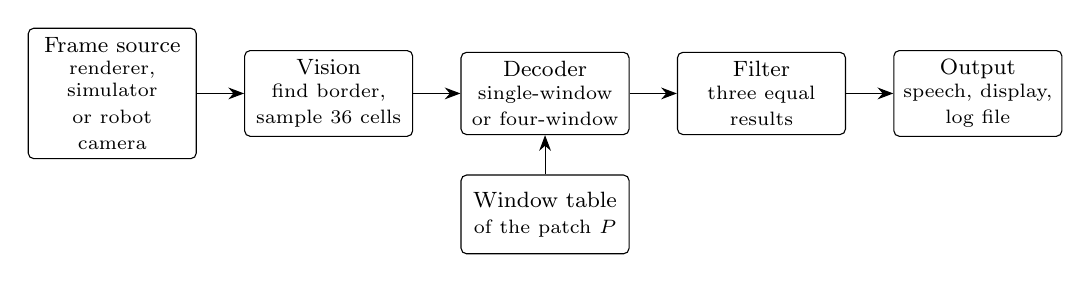
\begin{tikzpicture}[
  node distance=5mm and 6mm,
  box/.style={draw, rounded corners=2pt, align=center, font=\footnotesize, minimum height=10mm, text width=19mm},
  arr/.style={-{Stealth[length=2mm]}}]
\node[box] (src) {Frame source\\ \scriptsize renderer, simulator\\ \scriptsize or robot camera};
\node[box, right=of src] (vis) {Vision\\ \scriptsize find border,\\ \scriptsize sample 36 cells};
\node[box, right=of vis] (dec) {Decoder\\ \scriptsize single-window\\ \scriptsize or four-window};
\node[box, right=of dec] (st) {Filter\\ \scriptsize three equal\\ \scriptsize results};
\node[box, right=of st] (out) {Output\\ \scriptsize speech, display,\\ \scriptsize log file};
\node[box, below=of dec] (tab) {Window table\\ \scriptsize of the patch $P$};
\draw[arr] (src) -- (vis);
\draw[arr] (vis) -- (dec);
\draw[arr] (dec) -- (st);
\draw[arr] (st) -- (out);
\draw[arr] (tab) -- (dec);
\end{tikzpicture}
\caption{Design of the reading system.
The same vision stage and decoder are used for rendered images, for the simulator and for the robot.
A result is either a piece with its rotation or a rejection.}
\label{fig:pipeline}
\end{figure}


\section{Experiments}
\label{sec:experiments}

In this section we describe the experiments that address Question \ref{quest:reader}.
The design was fixed before the main data were collected.

\subsection{Design}
\label{sec:experiments_design}

Each experiment has two factors.
The first factor is the pattern, which is either strong-form or 4-orientable but not strong-form, with the same size.
The second factor is the decoder, which is either the single-window decoder or the four-window decoder.
Each read is classified as \emph{correct}, \emph{rejected} or \emph{wrong}, where a wrong read is an accepted read that reports an incorrect position or rotation.
Table \ref{tab:experiments} lists the three experiments.

\begin{table}[htbp]
\centering
\small
\begin{tabular}{@{}llll@{}}
\toprule
Experiment & Patterns & Windows & Reads \\
\midrule
Rendered puzzle & two $30$-by-$48$ patches & $5$-by-$5$ & $20{,}000$ per condition \\
Dense tori & two $6$-by-$6$ tori & $3$-by-$3$ & $20{,}000$ per condition \\
Robot & $40$ printed strong-form pieces & $5$-by-$5$ & approximately $320$ \\
\bottomrule
\end{tabular}
\caption{The planned experiments.
In the first two experiments one pattern is strong-form and the other is 4-orientable but not strong-form.
Every experiment is decoded with both decoders.}
\label{tab:experiments}
\end{table}

In the first experiment, a renderer draws a piece with a random rotation and a random perspective distortion, and then adds blur and noise.
The conditions vary the number of pixels per cell ($6$, $8$, $12$ and $24$), the tilt, the blur and the noise.

The second experiment is needed because the puzzle patterns are sparse.
The patch $P$ has $1{,}144$ windows, which is less than $0.02\%$ of the $2^{25}$ binary $5$-by-$5$ arrays, so a misread window is rarely equal to another window of either pattern.
The second experiment therefore uses tori of size $6$-by-$6$ with $3$-by-$3$ windows, in which a much larger fraction of all binary $3$-by-$3$ arrays occur as turned windows.
Each read is a $4$-by-$4$ patch, which contains four $3$-by-$3$ windows.
It has one condition with image noise and one condition in which exactly one cell of each read is changed.

In the third experiment, each of the $40$ printed pieces is held in front of the robot at eight rotations in steps of $45^\circ$.
Each frame is saved and is decoded afterwards with both decoders.

We make the following predictions.
\begin{enumerate}
\item On a strong-form pattern, no read with at most one misread cell is wrong, for either decoder. This follows from Proposition \ref{prop:reject}.
\item On the dense tori with exactly one changed cell, the single-window decoder produces wrong reads on the pattern that is not strong-form, and the four-window decoder rejects nearly all such reads on both patterns.
\item On the rendered puzzle, wrong reads are rare for both patterns and both decoders.
\item On the robot, the proportions of correct, rejected and wrong reads lie within the $95\%$ Wilson score intervals of the rendered proportions at the same number of pixels per cell.
\end{enumerate}
\todo{Add a  citation for the Wilson score interval.}

\subsection{Preliminary Results}
\label{sec:experiments_preliminary}

We implemented a prototype of the four-window decoder and tested it on the patch $P$.
There are $40 \cdot 4 \cdot 36 = 5{,}760$ ways to choose a piece, a rotation and one misread cell, and the decoder rejects all of them, as stated in Proposition \ref{prop:reject}.
It also decodes $2{,}000$ rendered images of pieces at random rotations correctly.

We repeated the first test on three random $30$-by-$48$ patches that are 4-orientable but not strong-form.
These patches contain $4$, $12$ and $4$ pairs of turned windows at distance $1$, respectively.
The four-window decoder again rejects all $5{,}760$ single misreads on each patch.
The single-window decoder reports a wrong position for at most $1$ of $4{,}000$ misread windows.
Therefore the puzzle alone does not separate the two patterns, which is the reason for the second experiment.

\todo{Report the three experiments, including the earlier simulation on complete tori.}

\subsection{Threats to Validity}
\label{sec:experiments_threats}

Rendered images may be easier to read than camera frames, which the third experiment is intended to measure.
The third experiment uses one robot and one room, and the pieces are positioned by hand.


\section{Final Remarks}
\label{sec:final}

\subsection{Summary}
\label{sec:final_summary}

In this paper we asked how large a binary torus can be if its windows must be distinguishable under quarter turns and must also allow a single misread cell to be detected.
We proved an upper bound that is half of the bound for 4-orientable tori when the window size is odd.
We determined the exact maximum of $36$ cells for $3$-by-$3$ windows, and we constructed a torus with $65{,}536$ cells for $5$-by-$5$ windows.
For $3$-by-$3$ windows the cost of error detection is larger than the counting bounds predict.
We also described a self-locating jigsaw puzzle and experiments that measure the effect of the pattern and of the decoder on a camera reader.

There are several potential criticisms of this work.
\begin{itemize}
  \item Theorems \ref{thm:exact3} and \ref{thm:exist5} are computational results. The unsatisfiable cases of Theorem \ref{thm:exact3} were confirmed by two programs but not by proof certificates.
  \item For $4$-by-$4$ and $5$-by-$5$ windows the lower and upper bounds are far apart, so Question \ref{quest:size} remains open for these sizes.
  \item The evidence that periodicity causes the additional loss is limited to $3$-by-$3$ windows.
  \item The jigsaw puzzle does not by itself show a benefit of the strong form, because the four-window decoder detects single misreads on patterns that are not strong-form.
\end{itemize}

\subsection{Additional Results}
\label{sec:final_additional}

The local search also found a 4-orientable binary torus of size $1152$-by-$1152$ with $5$-by-$5$ windows.
\todo{Report the decoding speed of the table lookup.}

\subsection{Additional Research}
\label{sec:final_research}

The jigsaw puzzle can be extended in several directions.
A puzzle with $1{,}000$ pieces requires $36{,}000$ cells, which fits within the $256$-by-$256$ torus.
The pieces could have interlocking tabs.
The pattern could be searched for directly as an open patch, since open patches for $3$-by-$3$ windows contain more turned windows than tori.
A pattern with distance $3$ would allow a single misread cell to be corrected.

\subsection{Open Problems}
\label{sec:final_open}

The following open problems are related to the work in this paper.
\begin{enumerate}
\item What is the maximum number of cells in a 4-orientable binary torus with $3$-by-$3$ windows? It is between $85$ and $120$.
\item What is the maximum number of cells in a strong-form binary torus with $4$-by-$4$ windows? It is between $441$ and $8{,}192$.
\item What is the maximum number of cells in a strong-form binary torus with $5$-by-$5$ windows? It is between $65{,}536$ and $4{,}193{,}280$.
\item Is there a strong-form torus that attains the bound in Theorem \ref{thm:bound} for some $u \geq 4$?
\item What is the maximum size of a strong-form open patch for each window size?
\item Is there a direct construction of large strong-form tori that does not rely on search?
\end{enumerate}

\subparagraph*{Acknowledgements.}
The jigsaw puzzle application was suggested by Dr Aaron Williams.

\subparagraph*{Use of AI tools.}
Anthropic's Claude models will be used to code and build the experiment with Reachy mini and for some programming behind the computational results.



\bibliography{refs.bib}
\bibliographystyle{plain}

\appendix

% \input{Assignment1.tex}
% \input{Assignment2.tex}
% \input{Assignment3.tex}
% \input{Assignment4.tex}

\section{Programs}
\label{sec:programs}

The Python package \texttt{otorus} contains the programs for the results in Sections \ref{sec:bounds} to \ref{sec:constructions}.
It includes the SAT encodings, the exhaustive search, the local search and a verifier for stored tori.
The Python package \texttt{jigsaw} contains the decoders, the renderer and the vision stage of Section \ref{sec:jigsaw}.

\todo{Add Python code using the \texttt{minted} package.}

\end{document}
